
\section{Introduction}

In recent years, the rapid growth of large language models (LLMs) 
\cite{Naveed2025} has intensified 
the trade-offs among computational throughput, memory capacity, and energy 
efficiency \cite{Gholami2024}. 
These challenges have driven the community to investigate low-precision 
data formats as a promising solution. 
Several emerging 8-bit formats, including FP8 \cite{Nvidia2022}, 
HiF8 \cite{Eric2025, Luo2024}, and MXFP8 \cite{Nvidia2025, AMD2025}, 
have already been deployed in commercial hardware products to accelerate 
deep learning workloads. 
Yet, as model sizes and context lengths continue to expand, the exploration 
of low-precision formats has naturally advanced toward the 4-bit frontier. 
Although MXFP8, as a Block Floating-Point (BFP) format, 
trades off performance for training stability, 
BFP currently appears to be the most practical pathway for 4-bit 
representation. 
Because further reductions in bit-width can only be 
realized by more effectively exploiting exponent redundancy within 
localized data.  
In the following, we examine 3 influential 4-bit BFP designs outlined 
in Figure \ref{BFP4-Structure},  
each representing a technical advancement and introducing a new perspective.

\begin{figure*}[htbp]
  \centering
  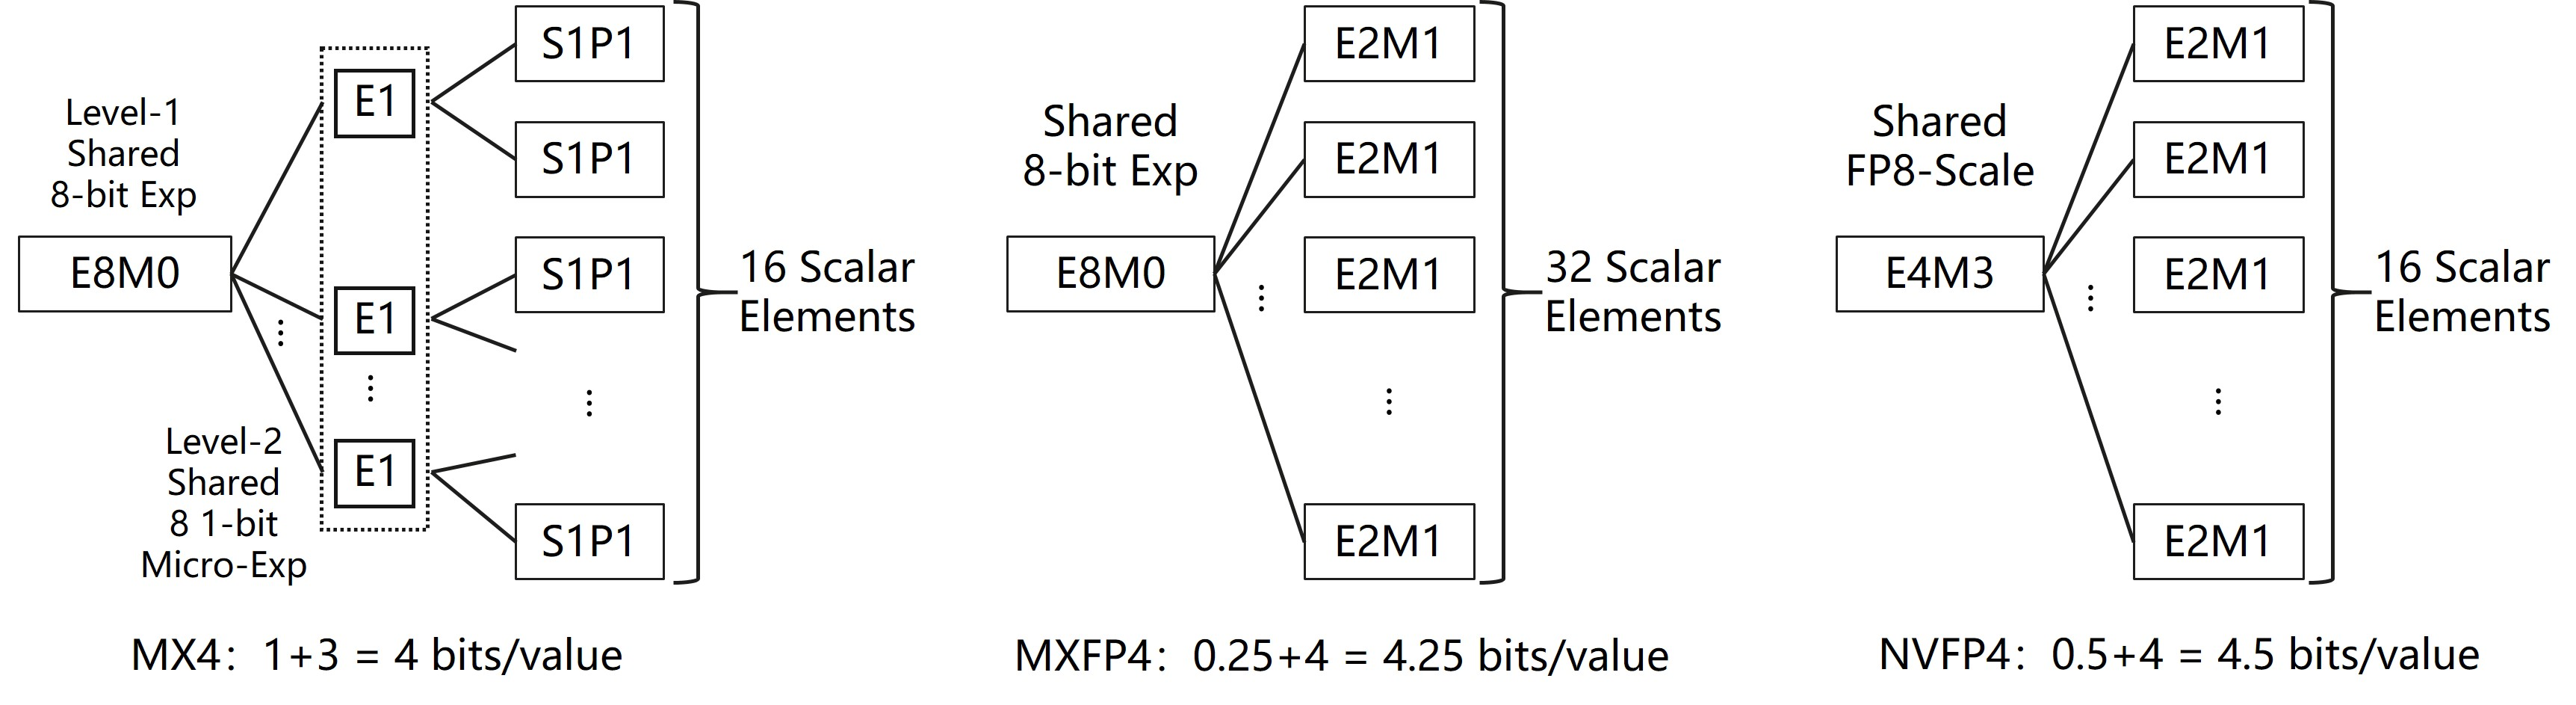
\includegraphics[width=17cm]{Fig/BFP4-Structure.jpg}
  \caption{The Structure of Three 4-bit Block Floating-Point Formats}
  \label{BFP4-Structure}
\end{figure*}

\noindent\textbf{MX4: Shared Micro-Exponents} \\
To characterize intra-group variation, Microsoft and Meta proposed the MX4 
format \cite{DarvishRouhani2023}, 
which augments the shared 8-bit exponent \cite{DarvishRouhani2020} with 
8-way 1-bit micro-exponents, 
forming a two-level hierarchical scaling structure. 
However, since MX4 uses a group size of 16,  
the metadata incurs a relatively high overhead of 1 bit per value. 
To keep the average storage below 5 bits per element, 
the in-group sign-magnitude format must be reduced from 4 to 3 bits, 
resulting in an average storage cost of 4 bits per value. 
This reduction ultimately causes MX4 to deliver even lower accuracy than 
the vanilla 4-bit BFP format \cite{DarvishRouhani2020}.  
Consequently, AMD's Versal AI Edge series adopted only the related MX6 and 
MX9 formats, abandoning MX4 \cite{AMD2024}. 
In summary, MX4 illustrates the conceptual value of shared micro-exponents 
for capturing intra-group variation, 
yet the metadata cost — exacerbated by the small group size — prevents the 
format from achieving practical accuracy and efficiency. 

\noindent\textbf{MXFP4: Individual Micro-Exponent} \\ 
OCP-MXFP4 assigns an individual 2-bit micro-exponent to each 
element, enabling finer intra-group variation \cite{Rouhani2023a}. 
Typically, the 4-bit in-group format is the sign-magnitude S1P2, 
where S denotes the sign bit, the 1 before P indicates a 1-bit integer part, 
and the 2 after P indicates a 2-bit fractional part (P is the binary point).
This is equivalent to the common E1M2 in floating-point style, where the 
sign bit is usually omitted. 
E1M2 provides at most 3-bit significand but only a limited dynamic range of 
log2(1.75/0.25) = 2.81 binades.  
MXFP4 replaces E1M2 with E2M1, sacrificing 1 bit significand to introduce 
a 2-bit micro-exponent, thereby expanding the dynamic range to 
log2(6/0.5) = 3.58 binades. 
The group size is also enlarged to 32, with an average storage cost of 4.25 
bits per value. 
MXFP4 has been adopted by several hardware vendors, including 
Nvidia \cite{Micikevicius2025}, AMD \cite{AMD2025}, and Huawei \cite{Eric2025}. 
However, it is now widely recognized that MXFP4 suffers from significant 
accuracy degradation when applied to both activations and weights 
\cite{Rouhani2023}. 
As a result, it is currently employed only for weight-only quantization, 
as in OpenAI's GPT-OSS \cite{Agarwal2025}, leaving the substantial 4-bit 
computing power unused. 
In summary, MXFP4 introduces a new trade-off between significand precision 
and intra-group dynamic range, 
but still fails to achieve the full potential of 4-bit BFP. 

\noindent\textbf{NVFP4: Floating-Point Scale} \\
In addition to MXFP4, the Blackwell architecture also supports a proprietary 
NVFP4 format, 
which leverages the advantages of E2M1 over E1M2 and introduces two changes 
\cite{Micikevicius2025}. 
First, power-of-two scale cannot guarantee to normalize each group's peak 
magnitude to the representable upper bound of E2M1, 
wasting intra-group dynamic range. 
NVFP4 replaces it with a fine-grained FP8-E4M3 floating-point scale, 
fully utilizing E2M1's expressive space. 
Second, NVFP4 adopts the same 16-element group size 
as MXF4 \cite{DarvishRouhani2023}, 
raising the average storage cost from 4.25 to 4.5 bits per value compared to 
MXFP4, but effectively reducing outlier-driven quantization error. 
Consequently, NVFP4 achieves better accuracy than MXFP4 and can be used for 
both weights and activations, 
thereby initially unlocking practical 4-bit BFP computing power. 
The benefits, however, come at two heavy costs. 
First, the dynamic range of E4M3 is not wide enough. 
NVFP4 requires additional software-based per-tensor scaling (PTS) for both 
inference \cite{Alvarez2025} and training \cite{Abecassis2025}, 
incurring performance degradation during format conversion. 
Second, when considering higher computing power compared to 8-bit formats, 
pairing a floating-point scale with a small group size leads to substantial 
area and power overhead in matrix-compute units. 
In summary, NVFP4 employs a floating-point scale to fully utilize the 
intra-group dynamic range, 
albeit with substantial hardware and software cost. 

From a comprehensive standpoint, the preceding analysis underscores the 
inherent complexity of designing a 4-bit BFP format. 
MX4 and MXFP4 characterize intra-group variation using distinct 
micro-exponent mechanisms, while NVFP4 further emphasizes the importance 
of maximizing intra-group dynamic range utilization. 
Each approach entails trade-offs across multiple design dimensions, 
such as metadata overhead, group size, significand precision, 
and both intra- and inter-group dynamic ranges. 
Despite the applicability of NVFP4 to both weights and activations, 
its limitations in accuracy, inter-group dynamic range, and hardware 
efficiency remain pronounced. 
These shortcomings highlight the ongoing challenge of realizing practical 
and efficient 4-bit BFP computation.

Through multiple rounds of analysis and iteration, 
we identified a suitable technical entry point and proposed a new 4-bit BFP 
format, HiF4. 
Compared with the state-of-the-art, HiF4 delivers higher accuracy, broader 
inter-group dynamic range suitable for both inference and training, 
and lower hardware cost. 
In this paper, we describe the specification of HiF4, including the format 
definition and conversion. 
We then present comparisons of quantization error and dot-product compute 
flow between different 4-bit BFP formats. 
Finally, extensive experimental results on LLM inference are 
reported to demonstrate the feasibility and advantages of HiF4.
